\documentclass[a4paper]{book}
\usepackage{a4wide}
\usepackage{makeidx}
\usepackage{fancyhdr}
\usepackage{graphicx}
\usepackage{multicol}
\usepackage{float}
\usepackage{textcomp}
\usepackage{alltt}
\usepackage{doxygen}
\usepackage[varg]{pxfonts}
\usepackage[linktocpage,
            pdfpagelabels,
            pagebackref=true,
            colorlinks=true,
            linkcolor=blue
           ]{hyperref}
\makeindex
\setcounter{tocdepth}{1}
\renewcommand{\footrulewidth}{0.4pt}
\makeatletter
\renewcommand{\l@section}{\@dottedtocline{1}{1.5em}{3.4em}}
\makeatother
\begin{document}
\begin{titlepage}
\vspace*{3cm}
\begin{center}
    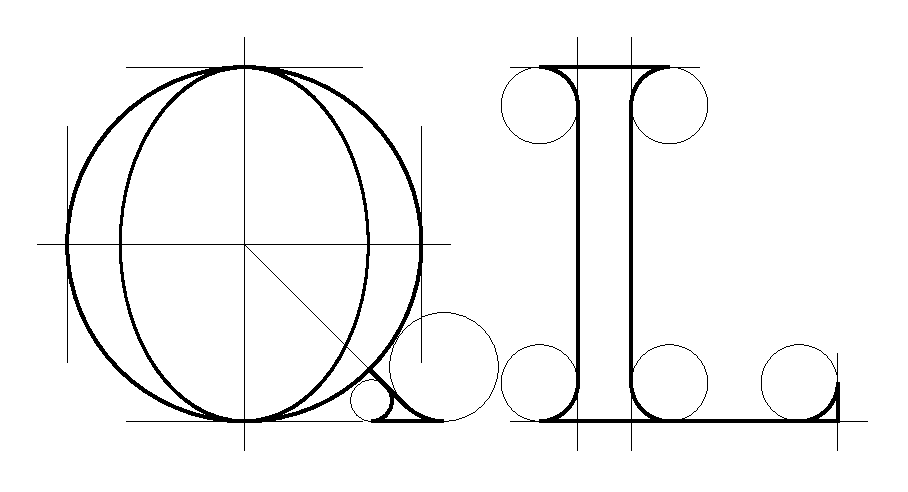
\includegraphics[width=10cm]{QL}\\
    {\Huge \bf QuantLib}\\
    \vspace*{0.5cm}
    {\LARGE \bf An open source library for quantitative finance}\\
    \vspace*{0.5cm}
    {\Large Version $projectnumber}\\
    \vspace*{5cm}
    {\large Generated by Doxygen $doxygenversion}\\
    \vspace*{0.5cm}
    {\small $date}\\
\end{center}
\end{titlepage}
\clearemptydoublepage
\pagenumbering{roman}
\tableofcontents
\clearemptydoublepage
\pagenumbering{arabic}

% User Manual

% User Manual
\hypertarget{usermanual}{}\part{User Manual}\label{usermanual}

\hypertarget{qlintro}{}\chapter{An introduction to QuantLib}\label{qlintro}
\input{index}
\include{overview}
\include{where}
\include{install}
\include{usage}
\include{platforms}
\include{history}
\include{todo}
\include{resources}
\include{group}
\include{license}

\hypertarget{frameworks}{}\chapter{QuantLib components}\label{components}
\input{coreclasses}
\include{datetime}
\include{lattices}
\include{findiff}
\include{mcarlo}
\include{fixedincome}
\include{currencies}
\include{instruments}
\include{math}
\include{patterns}
\include{termstructures}
\include{utilities}

\hypertarget{exlink}{}\chapter{Examples}\label{exlink}
More examples of using the QuantLib library can be found in
chapter~\ref{exchap} of the reference manual.
Should your viewer allow it, they can also be reached via the 
hyperlinks in the following list.
\input{examples}



% Reference manual - let Doxygen do its job
% page documentation will be removed by sed
\hypertarget{refmanual}{}\part{Reference Manual}\label{refmanual}

